\section{How many remain, and where to look}
\label{sec:survey}

\begin{figure*}[t]
\centering
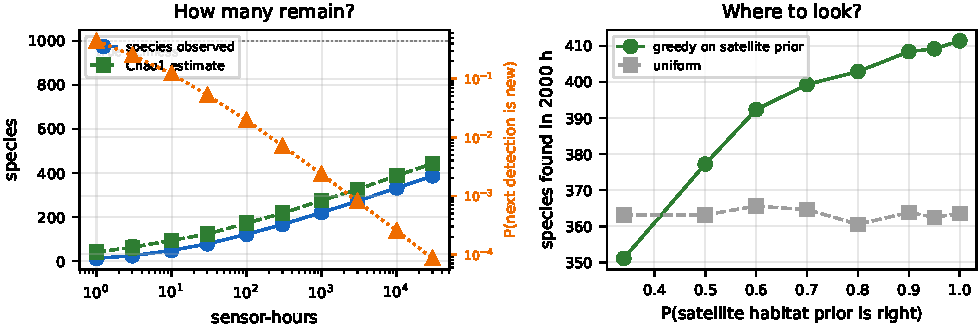
\includegraphics[width=\textwidth]{figures/survey.pdf}
\caption{Left: species observed and the Chao1 estimate of total richness
versus sensor-hours for a \SurS-species log-series community (mean $\pm$ s.e.\
over 30 replicates), with the Good--Turing probability that the next
detection is a new species (orange, right axis). Right: species found with a
\SurBudget\,h budget over 20 sites by a greedy allocation on a satellite
habitat prior versus a uniform survey, as the prior's reliability varies.}
\label{fig:survey}
\end{figure*}

\paragraph{How many remain.} A community of \SurS\ species with log-series
abundances is sampled by a sensor whose per-species detection rate scales
with abundance. After 10\,h it has seen \SurSeenTen\ species and Chao1
estimates \SurChaoTen\ $\pm$ \SurChaoSeTen; after 100\,h, \SurSeenHundred\
seen and \SurChaoHundred\ $\pm$ \SurChaoSeHundred; after 1000\,h,
\SurSeenThousand\ seen and \SurChaoThousand\ $\pm$ \SurChaoSeThousand; after
3000\,h, \SurSeenThreeK\ seen and \SurChaoThreeK\ $\pm$ \SurChaoSeThreeK\
(Figure~\ref{fig:survey}, left). Chao1 is a lower bound and behaves like one:
it rises with effort and stays well below the truth while most species are
still singletons, which is the regime the deep sea is in. The Good--Turing
discovery probability --- the chance that the \emph{next} detection is a species
not yet seen --- falls from \SurDiscTen\% at 10\,h to \SurDiscHundred\% at
100\,h and \SurDiscThousand\% at 1000\,h. That curve is the honest answer to
``can AI discover new species'': the sensor finds new ones fast at first, and
each further one costs exponentially more hours, whatever the classifier.

\paragraph{Where to look.} Twenty sites belong to a seamount habitat
(\SurRichSea\ species) or an abyssal plain (\SurRichPlain\ species); a
satellite-derived prior labels each site's habitat correctly with probability
$q$. A greedy rule spends the \SurBudget\,h budget where the expected marginal
number of new species under the prior is largest. When the prior is a coin
flip ($q=0.5$) greedy and uniform find the same \SurUniformHalf\ species;
at $q=0.7$ the gain is \SurGainSeven\%; at $q=0.9$ greedy finds \SurGreedyNine\
species against \SurUniformNine\ (\SurGainNine\%), and with a perfect prior
\SurGreedyTen\ against \SurUniformTen\ (\SurGainTen\%). The satellite cannot
see the animals, but a reliable map of where the rich habitat is buys a
sixth more discoveries per sensor-hour --- and an unreliable one buys
nothing, which is a reason to spend on bathymetry before spending on
hydrophones.
